\documentclass[a4paper]{article}
\usepackage{exercise}
%um nur aufgaben zu zeigen
%\usepackage[noanswer]{exercise} 
\usepackage{../images/preamble}
\usepackage{rotating}
\usetikzlibrary{decorations.pathmorphing}
\usetikzlibrary{decorations.markings}
\usetikzlibrary{arrows}
\usetikzlibrary{shapes.geometric}
\newcommand{\midarrow}{\tikz \draw[-triangle 90] (0,0) -- +(.02,0);}
\usepackage{xcolor}
%\usepackage{draftwatermark}
%\SetWatermarkText{\textsc{Draft 2}}
%\SetWatermarkScale{3}
%\SetWatermarkColor{red!30}

\usepackage[printwatermark]{xwatermark}
\newsavebox\mybox
\savebox\mybox{\tikz[color=red,opacity=0.3]\node{\textsc{Entwurf}};}
\newwatermark*[
allpages,
angle=45,
scale=10,
xpos=-4cm,
ypos=4cm
]{\usebox\mybox}
\pagestyle{fancy}
\fancyhead[L]{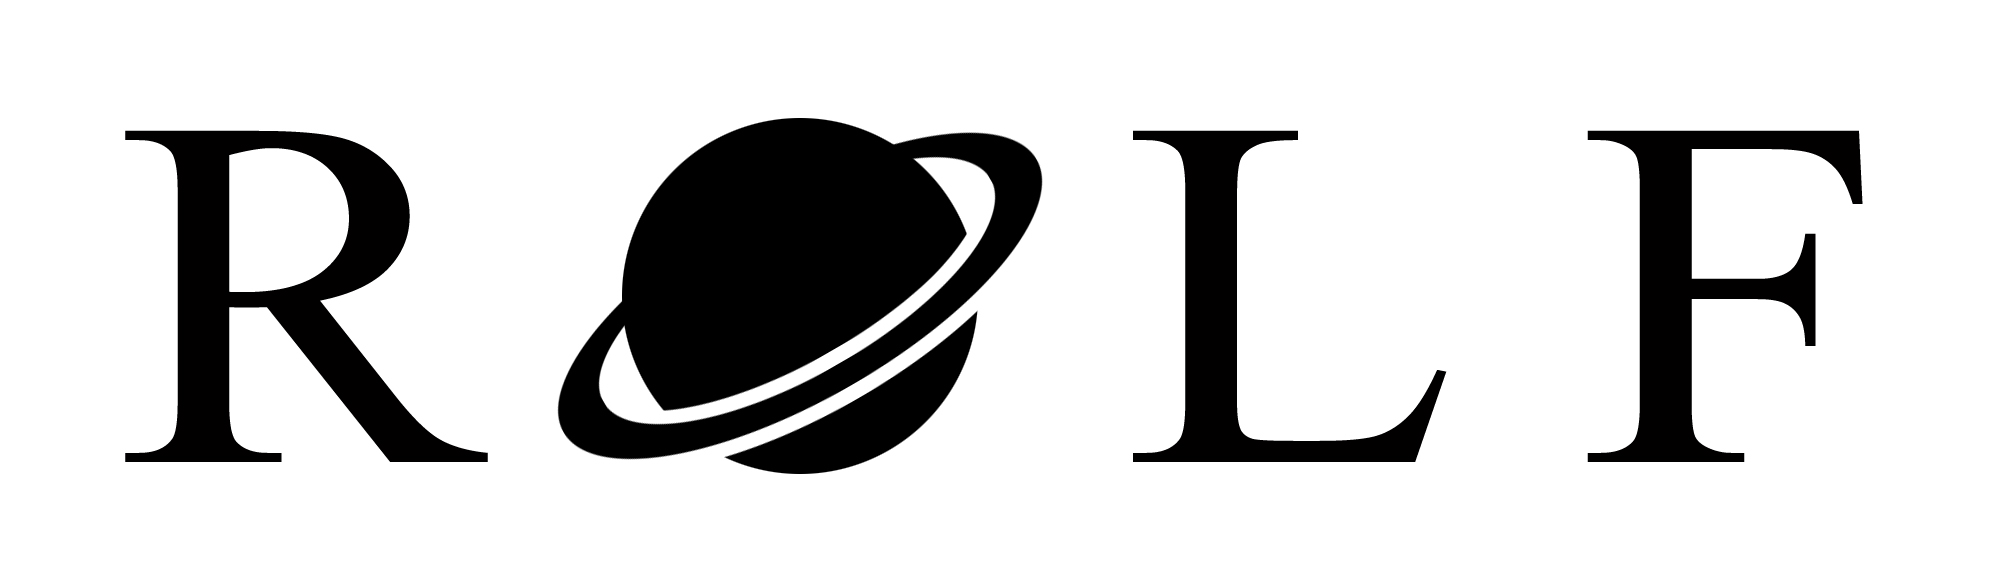
\includegraphics[width=2cm]{../images/rolfal.jpg}}
\fancyhead[R]{\textsc{Lösung Aufgabenserie 4}}

\makeatletter
\newcommand{\asti}{%
	\check@mathfonts
	\leavevmode
	{\ooalign{%
			\hidewidth
			\raisebox{1.2ex}{\fontsize{\ssf@size}{0}\selectfont $\heartsuit$}%
			\hidewidth\cr
			\i\cr
		}}%
	}
	\makeatother


\begin{document}
	\vspace*{-1cm}
	\parbox{4cm}{\vspace{-0.2cm}\hspace{5cm}}
	\parbox{10.6cm}{\setstretch{2.0} \centering{ \huge \textsf{Phys\asti k für Len\asti
			}}\\
			Abgabe: 5. Oktober \\ \vspace*{-.5cm} }
		\vspace{0.5cm}

\thispagestyle{empty}


\noindent

\begin{Exercise}[label = kin, title = Kinematik]
	Jedes normales Physikbuch fängt damit an, dass es dir etwas über Bewegungen beibringt. Das ist auch ziemlich schlau, weil Physik sich eigentlich immer damit beschäftigt, wann sich Sachen bewegen, oder eben auch nicht.\\
	\asti


\end{Exercise}




\end{document}